
\chapter{Optimizing Program Performance}

\begin{enumerate}
    \item select an appropriate set of algorithms and data structures
    \item  write source code that the compiler can effectively optimize to turn into efficient executable code
    \item  divide a task into portions that can be computed in parallel, on some combination of multiple cores and multiple processors.
\end{enumerate}
명심할것. 두번째를 이해하기위해 컴파일러의 능력과 한계를 알아야한다. 최적화를 위하면서도 코드 가독성은 유지해야한다.


\section{Capabilities and Limitations of Optimizing Compilers}


컴파일러 최적화 명령어는 -0g -1g -2g ... 이 있다.


다음 두개의 코드가 있다고 생각해보자 
\begin{lstlisting}[style = CStyle]
void twiddle1(long *xp, long *yp)
{
*xp += *yp;
*xp += *yp;
}

void twiddle2(long *xp, long *yp)
{
*xp += 2* *yp;
}
\end{lstlisting}
twiddle1은 twiddle2로 최적화 될수있는가? 답은 아니 다. xp와 yp가 동일하다고 생각해보자. 그러면 명확할 것이다.


\begin{lstlisting}[style = CStyle]
long f();
long func1() {
return f() + f() + f() + f();
}

long func2() {
return 4*f();
}
\end{lstlisting}
func1 이 func2로 최적화 될 수 있다고 생각한다. 하지만 f에서 전역변수를 건든다고 생각해보자 4번 바뀔게 한번만 바뀌는 일이 될것이다.

컴파일러는 위험요소가 있을경우 최적화를 하지않는다.

\section{Eliminating Loop Inefficiencies}

\begin{lstlisting}[style = CStyle]
void combine1(vec_ptr v, data_t *dest)
 {
 long i;

 *dest = IDENT;
 for (i = 0; i < vec_length(v); i++) {
 data_t val;
 get_vec_element(v, i, &val);
 *dest = *dest OP val;
 }
 }

\end{lstlisting}

이게 어떻게 성능 개선이되는지 보자.

\begin{lstlisting}[style = CStyle]
void combine2(vec_ptr v, data_t *dest)
 {
 long i;
 long length = vec_length(v);

 *dest = IDENT;
 for (i = 0; i < length; i++) {
 data_t val;
 get_vec_element(v, i, &val);
 *dest = *dest OP val;
 }
 }
\end{lstlisting}


\begin{figure}[h!]
    \centering
    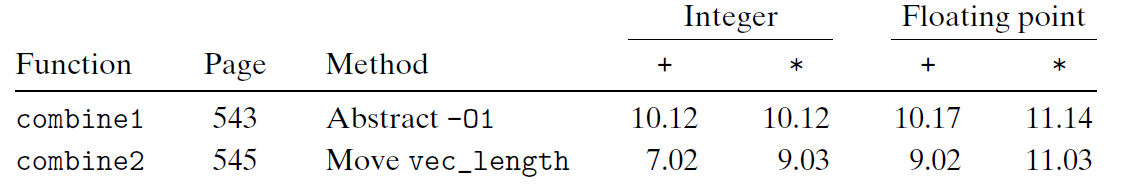
\includegraphics[scale=0.4]{pic/section5/pic1}
\end{figure}



\begin{lstlisting}[style = CStyle]
/* Convert string to lowercase: slow */
void lower1(char *s)
{
    long i;

    for (i = 0; i < strlen(s); i++)
        if (s[i] >= `A' && s[i] <= 'Z')
            s[i] -= ('A' - 'a');    
}

/* Convert string to lowercase: faster */
void lower2(char *s)
{
    long i;
    long len = strlen(s);

    for (i = 0; i < len; i++)
        if (s[i] >= `A' && s[i] <= 'Z')
            s[i] -= (`A' - 'a');
}

/* Sample implementation of library function strlen */
/* Compute length of string */
size_t strlen(const char *s)
{
    long length = 0;
    while (*s != '\0') {
        s++;
        length++;
    }
    return length;
}
\end{lstlisting}

\begin{figure}[h!]
    \centering
    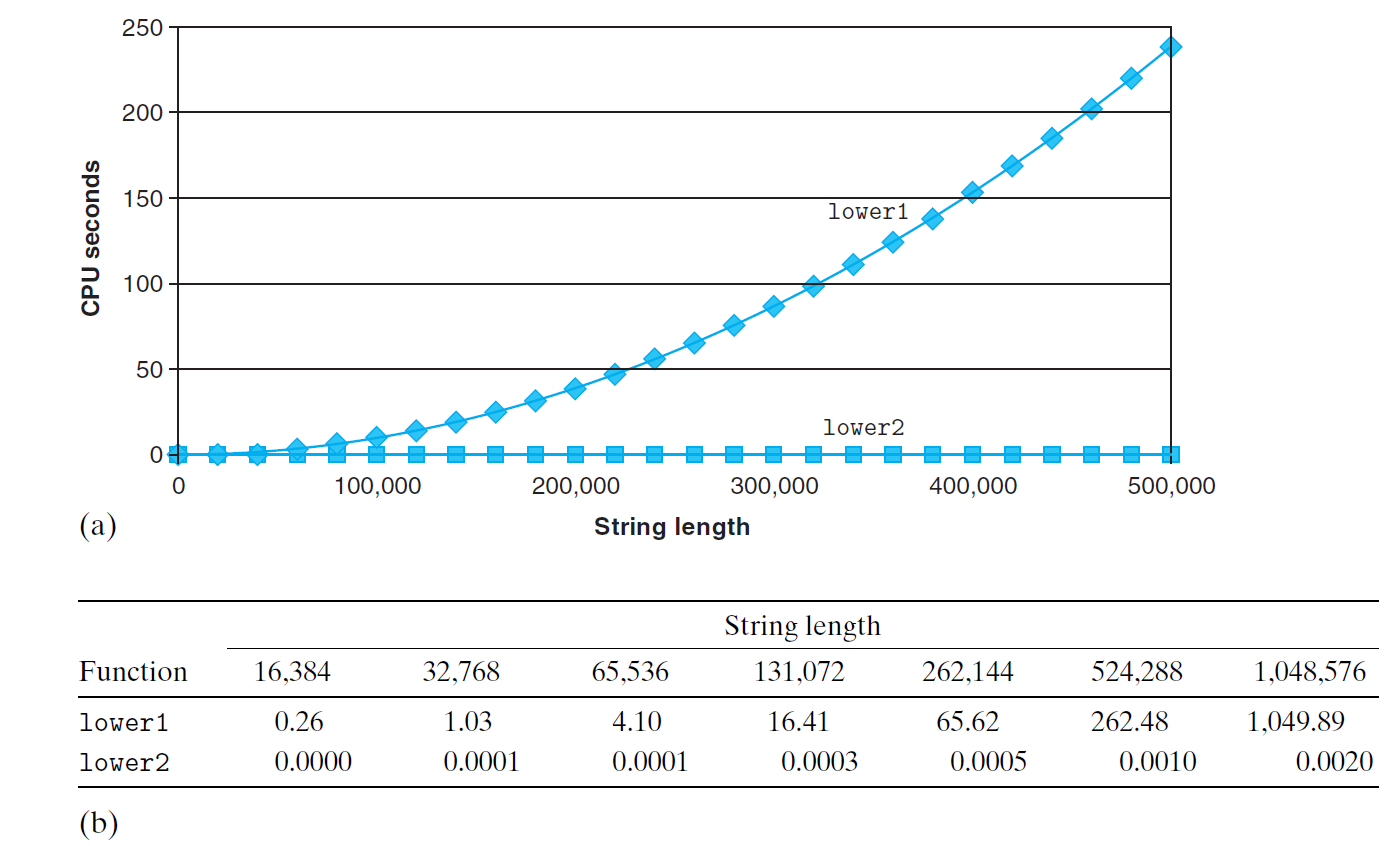
\includegraphics[scale=0.4]{pic/section5/pic2}
    \caption{lower 성능비교}
\end{figure}

시간복잡도 계산으로도 충분히 알 수 있다.
문자열 길이가 변하는게 아니라면 strlen을 반복문안에 넣는 짓은 하지말자.

\section{Reducing Procedure Calls}

\begin{lstlisting}[style = CStyle]
void combine3(vec_ptr v, data_t *dest)
{
    long i;
    long length = vec_length(v);
    data_t *data = get_vec_start(v);
    *dest = IDENT;
    for (i = 0; i < length; i++) {
    *dest = *dest OP data[i];
    }
}
\end{lstlisting}

대충 함수안에서 계속 함수를 쳐부르는 짓은 오버헤드와 불리는 함수안에서 처리하는 불필요한 작업으로 느려진다는 뜻.
근데 뒤에 더다룬다함


\begin{figure}[h!]
    \centering
    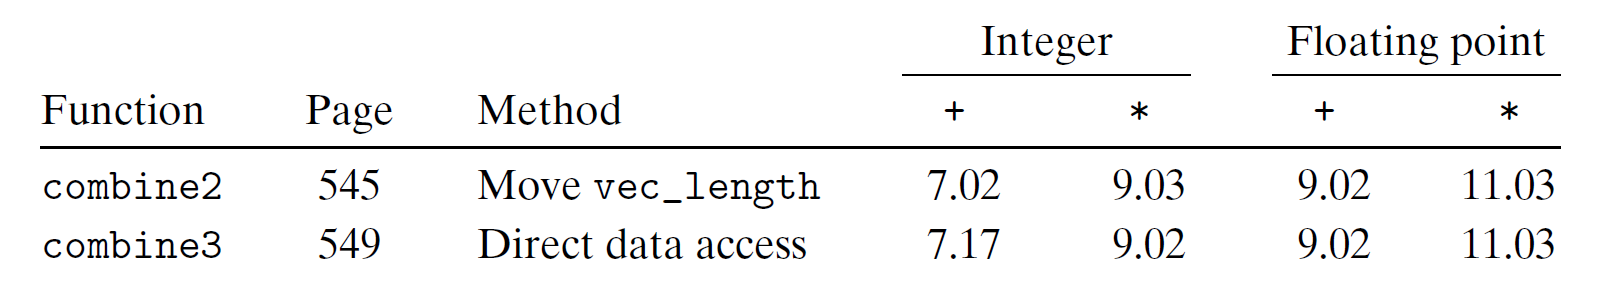
\includegraphics[scale=0.3]{pic/section5/pic3}
\end{figure}

\section{Eliminating Unneeded Memory References}

combine3에서 내부 루프는 포인터 dest가 메모리 참조를 계속하는 식이다.
다음 방식이 조금더 효율적이다.

\begin{lstlisting}[style = CStyle]
void combine4(vec_ptr v, data_t *dest)
 {
 long i;
 long length = vec_length(v);
 data_t *data = get_vec_start(v);
 data_t acc = IDENT;

for (i = 0; i < length; i++) {
 acc = acc OP data[i];
 }
 *dest = acc;
 }
\end{lstlisting}




\begin{figure}[h!]
    \centering
    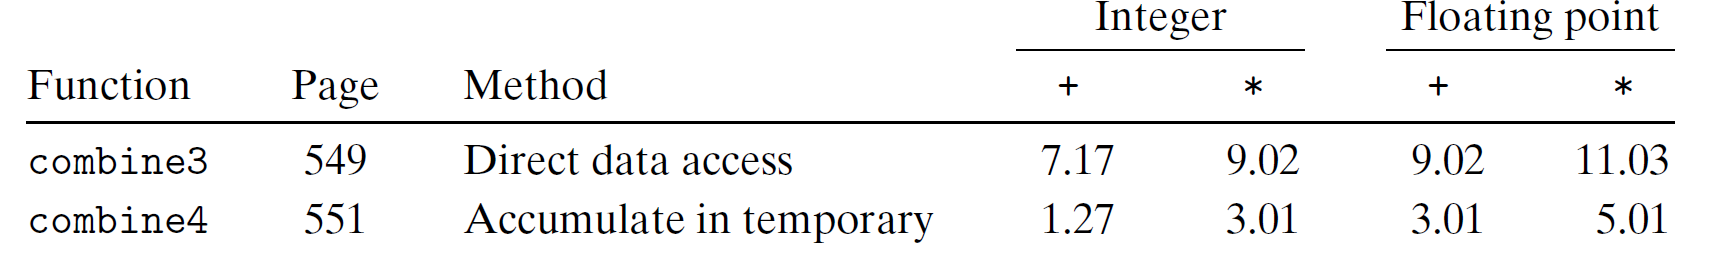
\includegraphics[scale=0.3]{pic/section5/pic4}
\end{figure}



\section{Understanding Modern Processors}

아몰랑


\section{Loop Unrolling}

while의 작동방식을 어셈블리로 한번보면 
if와  goto를 합쳐놓은 방식이다.
if는 단일 연산에비해느림 따라서
if검사를 적게 하게하면(=반복되는 횟수를 줄이면) 성능개선이 이루어진다.

\begin{lstlisting}[style = CStyle]
/* 2 x 1 loop unrolling */
void combine5(vec_ptr v, data_t *dest)
    {
    long i;
    long length = vec_length(v);
    long limit = length-1;
    data_t *data = get_vec_start(v);
    data_t acc = IDENT;

    /* Combine 2 elements at a time */
    for (i = 0; i < limit; i+=2) {
    acc = (acc OP data[i]) OP data[i+1];
    }

    /* Finish any remaining elements */
    for (; i < length; i++) {
    acc = acc OP data[i];
    }
    *dest = acc;
}
\end{lstlisting}


\begin{figure}[h!]
    \centering
    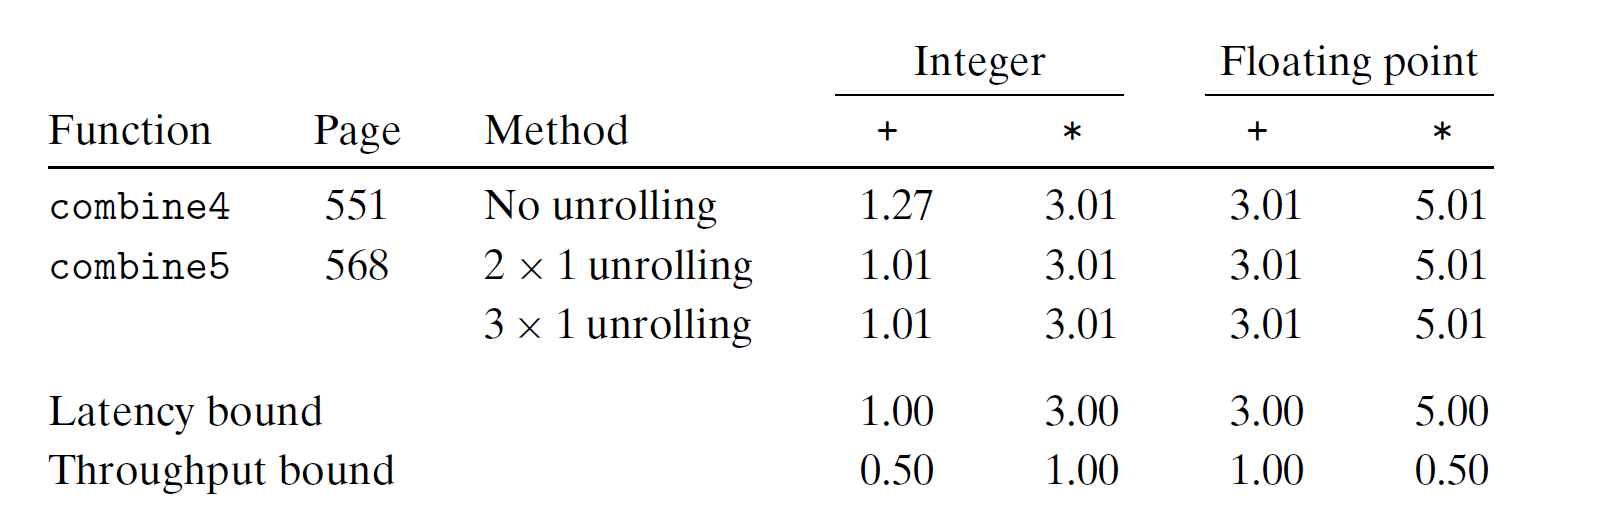
\includegraphics[scale=0.3]{pic/section5/pic5}
\end{figure}


\begin{figure}[h!]
    \centering
    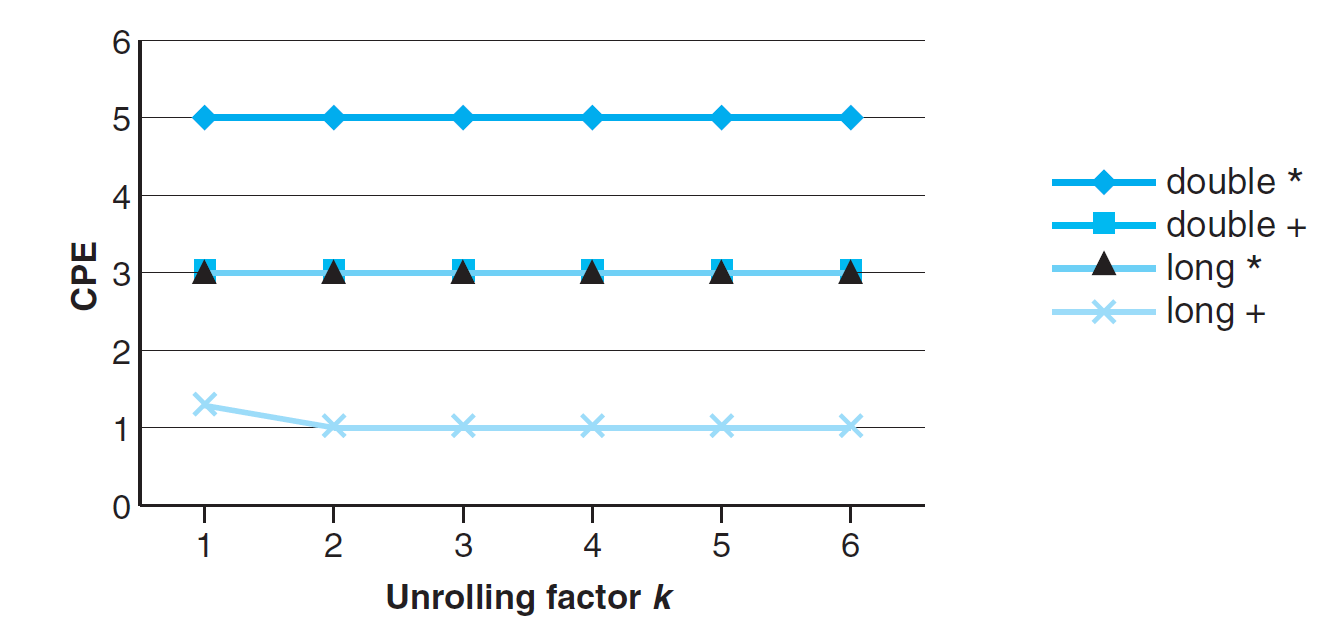
\includegraphics[scale=0.4]{pic/section5/pic6}
    \caption{ kx1 에따른 성능비교}
\end{figure}


이 생각을 할수있다.
루프풀기를 최대로하면 제일 좋은게아닌가?

여러단점이있다.

\url{http://z3moon.com/프로그래밍/loop_unrolling}

\url{https://en.wikipedia.org/wiki/Loop_unrolling}

\begin{enumerate}
    \item 코드 크기 증가
    \item 가독성 저해
    \item 함수호출이 있을 경우 캐시 미스율 향상
\end{enumerate}

연산이 복잡해질수록 인덱스의 계산과 if조건이 수행시간에 영향을 주지않는다.
for문 내부가 간단한 코드일때 가장 효과가 좋다.

\section{Enhancing Parallelism}

\subsubsection{Multiple Accumulators}
연산을 나눠서 계산하고 마지막에 합치는 방식

\begin{lstlisting}[style = CStyle]
/* 2 x 2 loop unrolling */
void combine6(vec_ptr v, data_t *dest)
{
    long i;
    long length = vec_length(v);
    long limit = length-1;
    data_t *data = get_vec_start(v);
    data_t acc0 = IDENT;
    data_t acc1 = IDENT;

    /* Combine 2 elements at a time */
    for (i = 0; i < limit; i+=2) {
    acc0 = acc0 OP data[i];
    acc1 = acc1 OP data[i+1];
    }

    /* Finish any remaining elements */
    for (; i < length; i++) {
    acc0 = acc0 OP data[i];
    }
    *dest = acc0 OP acc1;
}
\end{lstlisting}

\begin{figure}[h!]
    \centering
    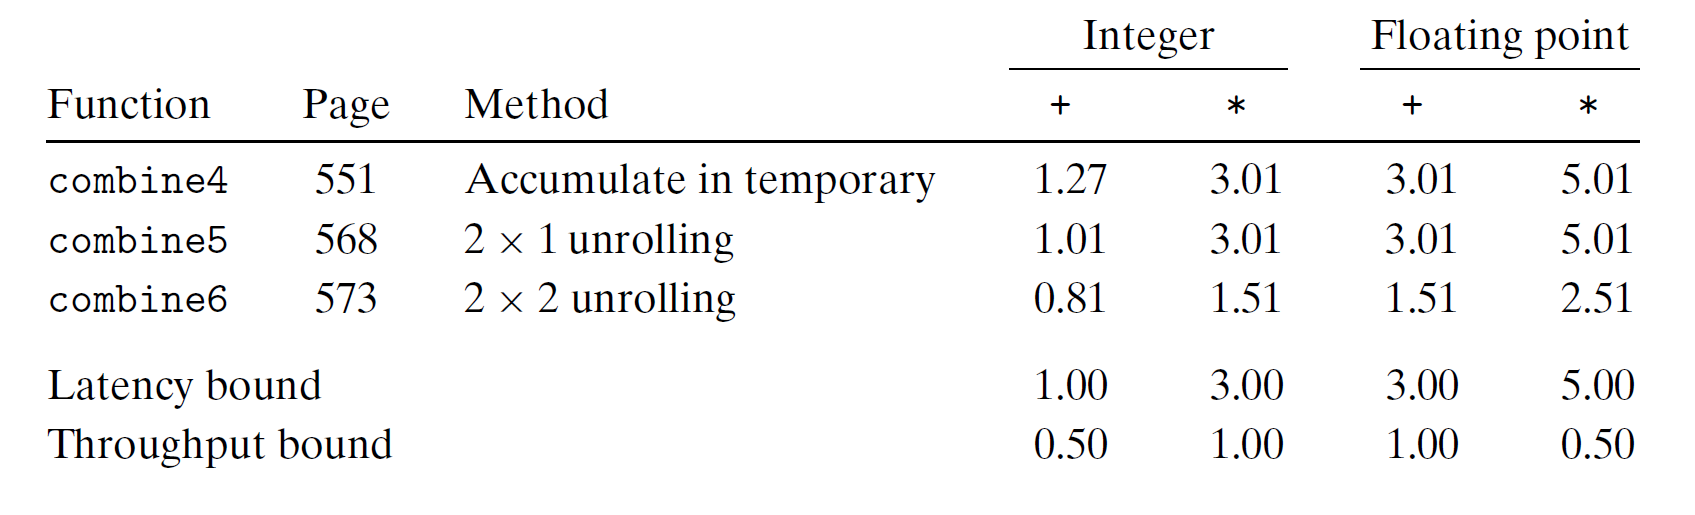
\includegraphics[scale=0.3]{pic/section5/pic7}
\end{figure}



\begin{figure}[h!]
    \centering
    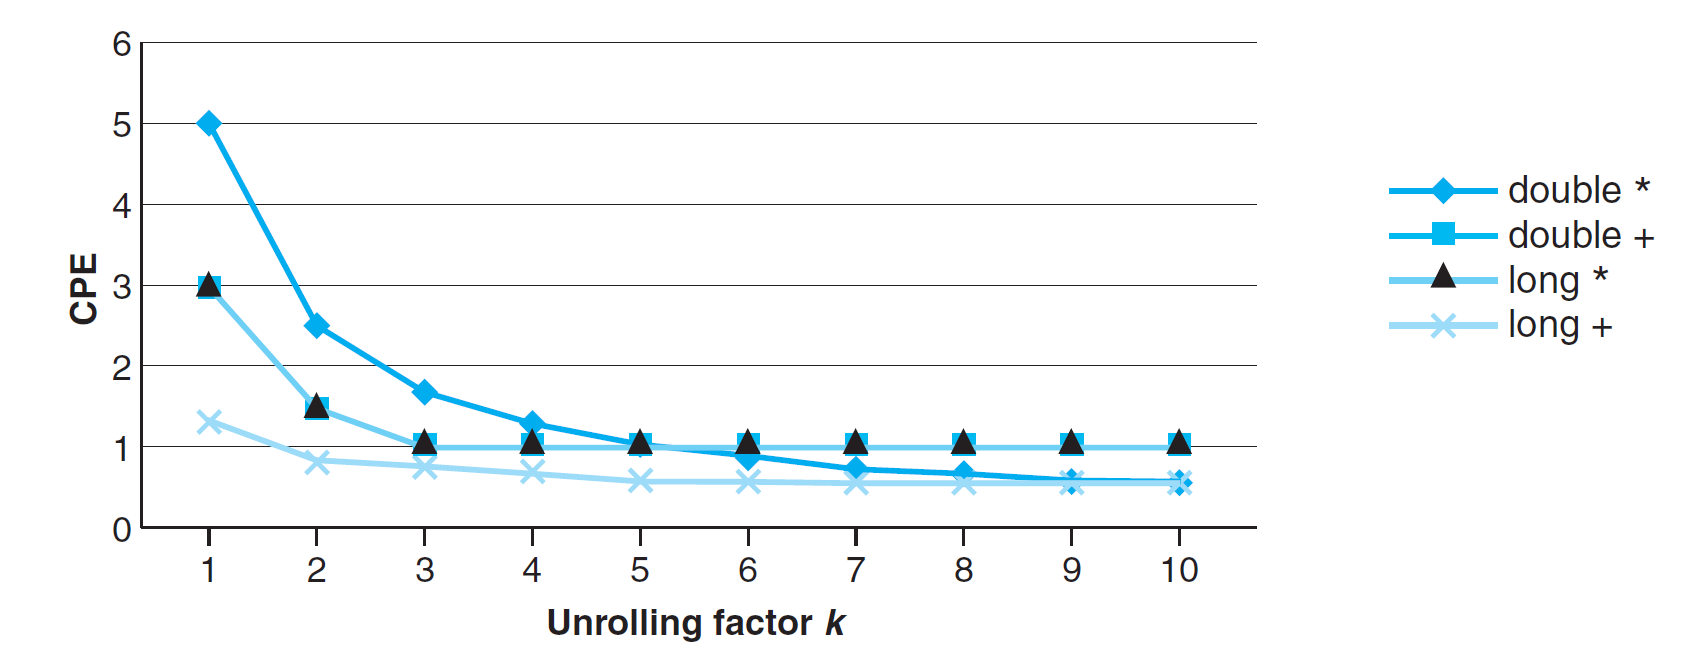
\includegraphics[scale=0.3]{pic/section5/pic8}
    \caption{kxk}
\end{figure}


\subsubsection{Reassociation Transformation}


\begin{lstlisting}[style = CStyle]
/* 2 x 1a loop unrolling */
void combine7(vec_ptr v, data_t *dest)
{
long i;
long length = vec_length(v);
long limit = length-1;
data_t *data = get_vec_start(v);
data_t acc = IDENT;

/* Combine 2 elements at a time */
for (i = 0; i < limit; i+=2) {
acc = acc OP (data[i] OP data[i+1]);
}

/* Finish any remaining elements */
for (; i < length; i++) {
acc = acc OP data[i];
}
*dest = acc;
}
\end{lstlisting}

combine5의 다음코드를


\begin{lstlisting}[style = CStyle]
    acc = (acc OP data[i]) OP data[i+1];
\end{lstlisting}


\begin{lstlisting}[style = CStyle]
    acc = acc OP (data[i] OP data[i+1]);
\end{lstlisting}
로 바꾼다.

\begin{figure}[h!]
    \centering
    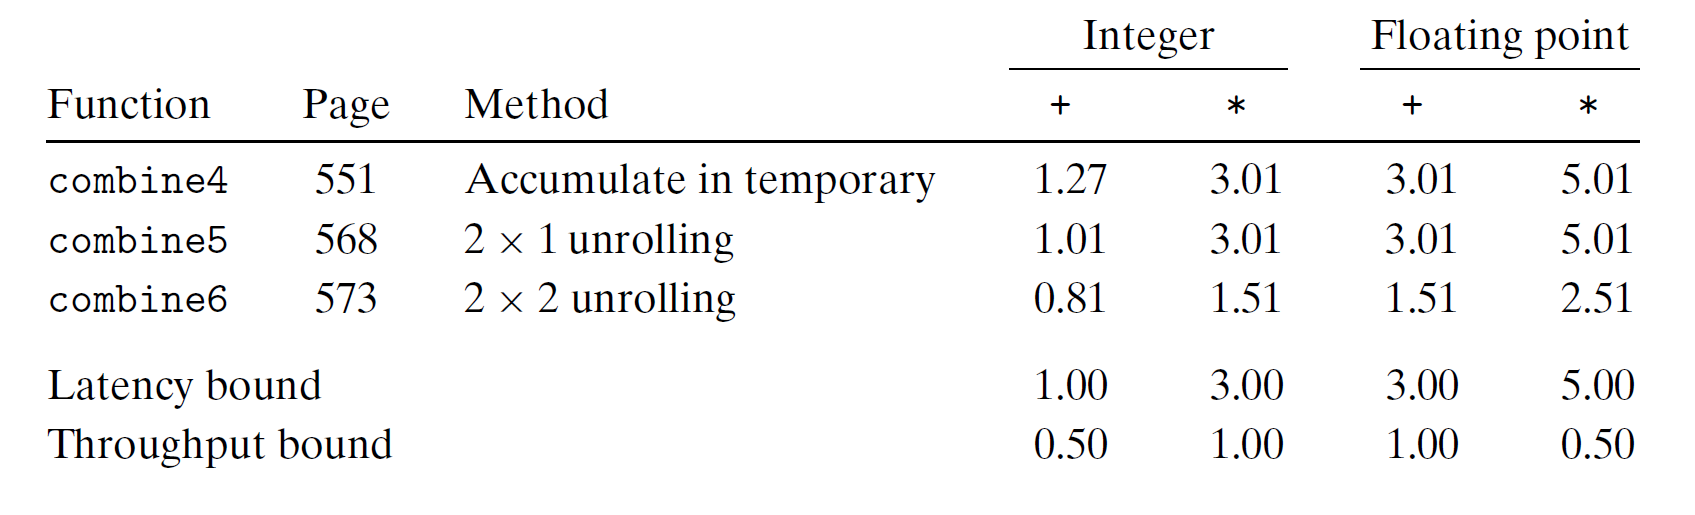
\includegraphics[scale=0.3]{pic/section5/pic7}
    \caption{}
\end{figure}



\begin{figure}[h!]
    \centering
    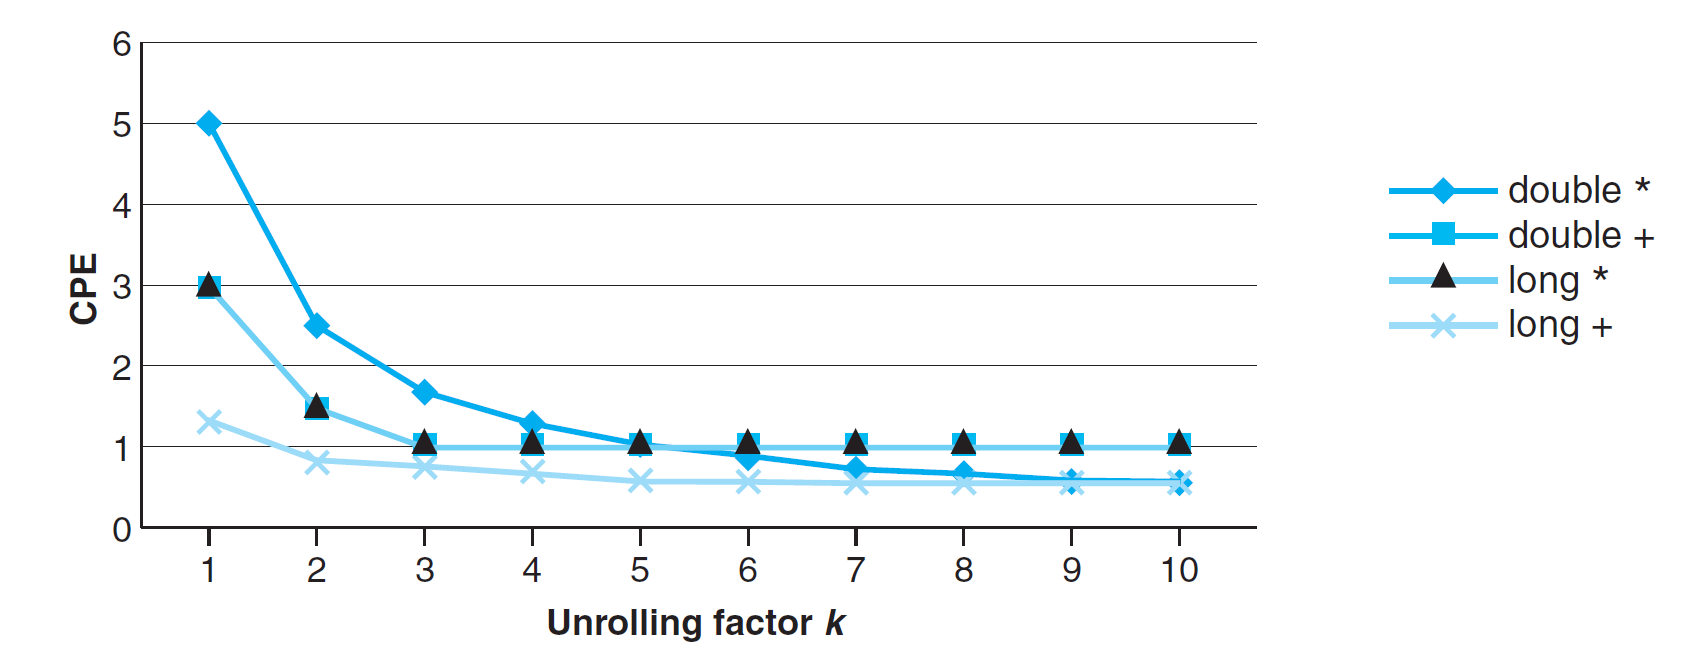
\includegraphics[scale=0.3]{pic/section5/pic8}
    \caption{}
\end{figure}


